\documentclass[
]{beamer}

\usepackage[english]{babel}
\usepackage[utf8]{inputenc}
\usepackage[T1]{fontenc}
\usepackage{csquotes}
\usepackage{biblatex}
\usepackage{hyperref}
\hypersetup{
    colorlinks=true,
    linkcolor=blue,
    filecolor=magenta,      
    urlcolor=cyan,
}
\addbibresource{example.bib}
\usepackage{booktabs}
\usetheme{Pittsburgh}
\setbeamertemplate{caption}[numbered]

\title[Short Presentation Title]{Clustering BNP data with von Mises-Fisher distributions.}
\subtitle[Short Presentation Subtitle]{Plus code base and options for future development.}
\author[E. Vacek]{Everett Vacek}
%\institute[University Center Telč MU]{University Center Telč, Masaryk University}
\date{\today}
\subject{Presentation Subject}
\keywords{von Mises-Fisher, clustering, bionanoprobe}
\begin{document}

\begin{frame}[plain]
\maketitle
\end{frame}

\section[Short Section 1 Name]{Full Section 1 Name}
\subsection[Short Subsection 1 Name]{Full Subsection 1 Name}

% page 3
\subsection[movMF image]{Mixture of vMF distributions on the 3-sphere}
\begin{frame}{von Mises-Fisher distributions.}
\begin{figure}[h]
  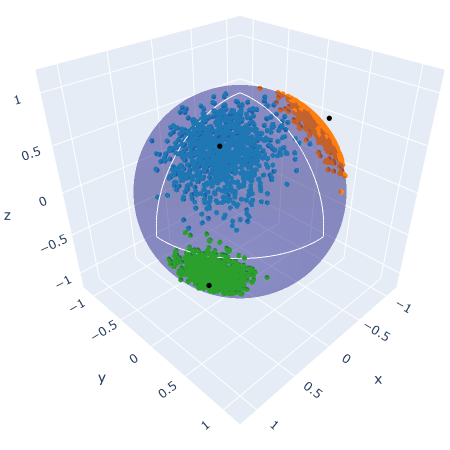
\includegraphics[width=.5\textwidth,height=.5\textheight,keepaspectratio]{vMF.png}
  \caption{Mixture of three von Mises Fisher distributions on the 3-sphere. Black spots are above $\boldsymbol{\mu}$ for each distribution. White triangle is the positive octant.
  }
\end{figure}
\end{frame}

% page 2
\begin{frame}{von Mises Fisher distributions}%{Subtitle}
Random vector $\boldsymbol{x}$ has a $d$-variate von Mises-Fisher (vMF) distribution if its probability density function is given by:
$$f(\boldsymbol{x}|\boldsymbol{\mu}, \kappa) = c_d(\kappa)e^{\kappa\boldsymbol{\mu}^T\mathbf{x}}$$
\begin{itemize}
  \item $\boldsymbol{x}$: random d-dimensional unit vector (i.e. $||\boldsymbol{x}|| = 1$).
  \item $\boldsymbol{\mu}$: mean direction of distribution. Also a unit vector.
  \item $\kappa$: concentration parameter.
  \begin{itemize}
    \item For $\kappa = 0$, distribution becomes uniform distribution on unit sphere. For $\kappa = \infty$, distribution becomes single point.
  \end{itemize}
  \item $c_d(\kappa)$: normalizing parameter. Given by,
  $$c_d(\kappa) = \frac{\kappa^{d/2-1}}{(2\pi)^{d/2}I_{d/2-1}(\kappa)}$$
  \begin{itemize}
      \item $I_r(\cdot)$: modified Bessel function of the first kind and order r.
  \end{itemize}
\end{itemize}
\end{frame}

%page 8
\begin{frame}{Why vMF not Gaussians?}
\begin{figure}[h]
  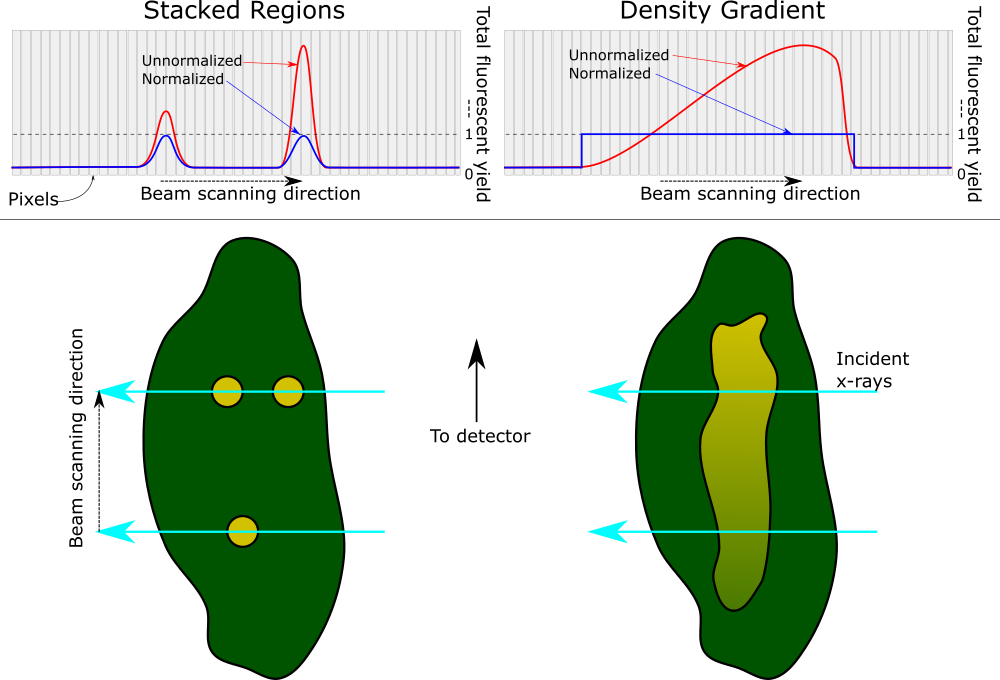
\includegraphics[width=1\textwidth,height=.5\textheight,keepaspectratio]{Normalization.png}
  \caption{In a 2D XRF projection increasing brightness may be due to overlapping regions or regions with higher concentration making it difficult to discern between the two. Because of this I chose to normalize the data and cluster only based on element composition, not concentration.}
\end{figure}
\end{frame}

%page 4
\subsection[Short Subsection 3 Name]{Full Subsection 3 Name}

\begin{frame}{Bionanoprobe Data.}
\begin{figure}[h]
  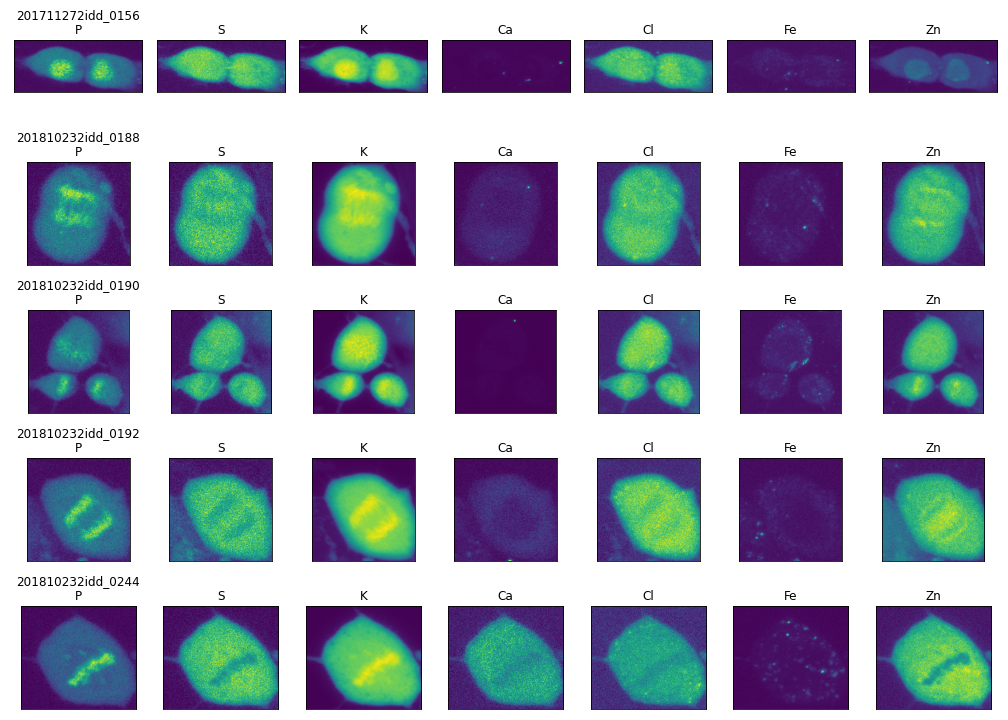
\includegraphics[width=1\textwidth,height=.7\textheight,keepaspectratio]{unmasked.png}
  \caption{XRF images of mouse fibroblasts.
  }
\end{figure}
\end{frame}

\begin{frame}{Masked Bionanoprobe Data.}
\begin{figure}[h]
  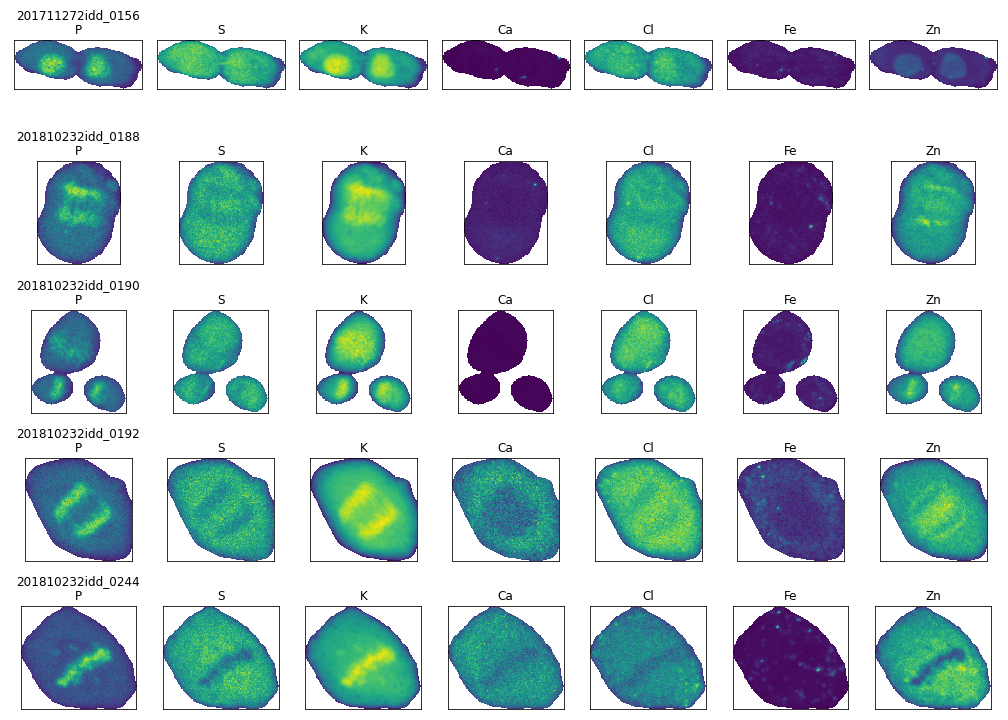
\includegraphics[width=1\textwidth,height=.7\textheight,keepaspectratio]{masked.png}
  \caption{After using morphological filters to mask data.
  }
\end{figure}
\end{frame}

%page 5
\begin{frame}{Prepossessing BNP data}
For BNP data each pixel is its own d-dimensional elemental concentration vector, 
$$\boldsymbol{X_p} = (X_1, X_2, ..., X_d).$$
Each component, $X_i$, is that elements concentration for a given pixel and has units $\mu g/cm^2$. 

\begin{itemize}
    \item The variance will vary for each element! But, vMF is univariate and expect normal distributions. We must scale our data using a to such that each dimension has the same variance. Robust scaler preprocessing rescales element values to the interquartile range.
\end{itemize}
    
\end{frame}

\begin{frame}{Pandas}
    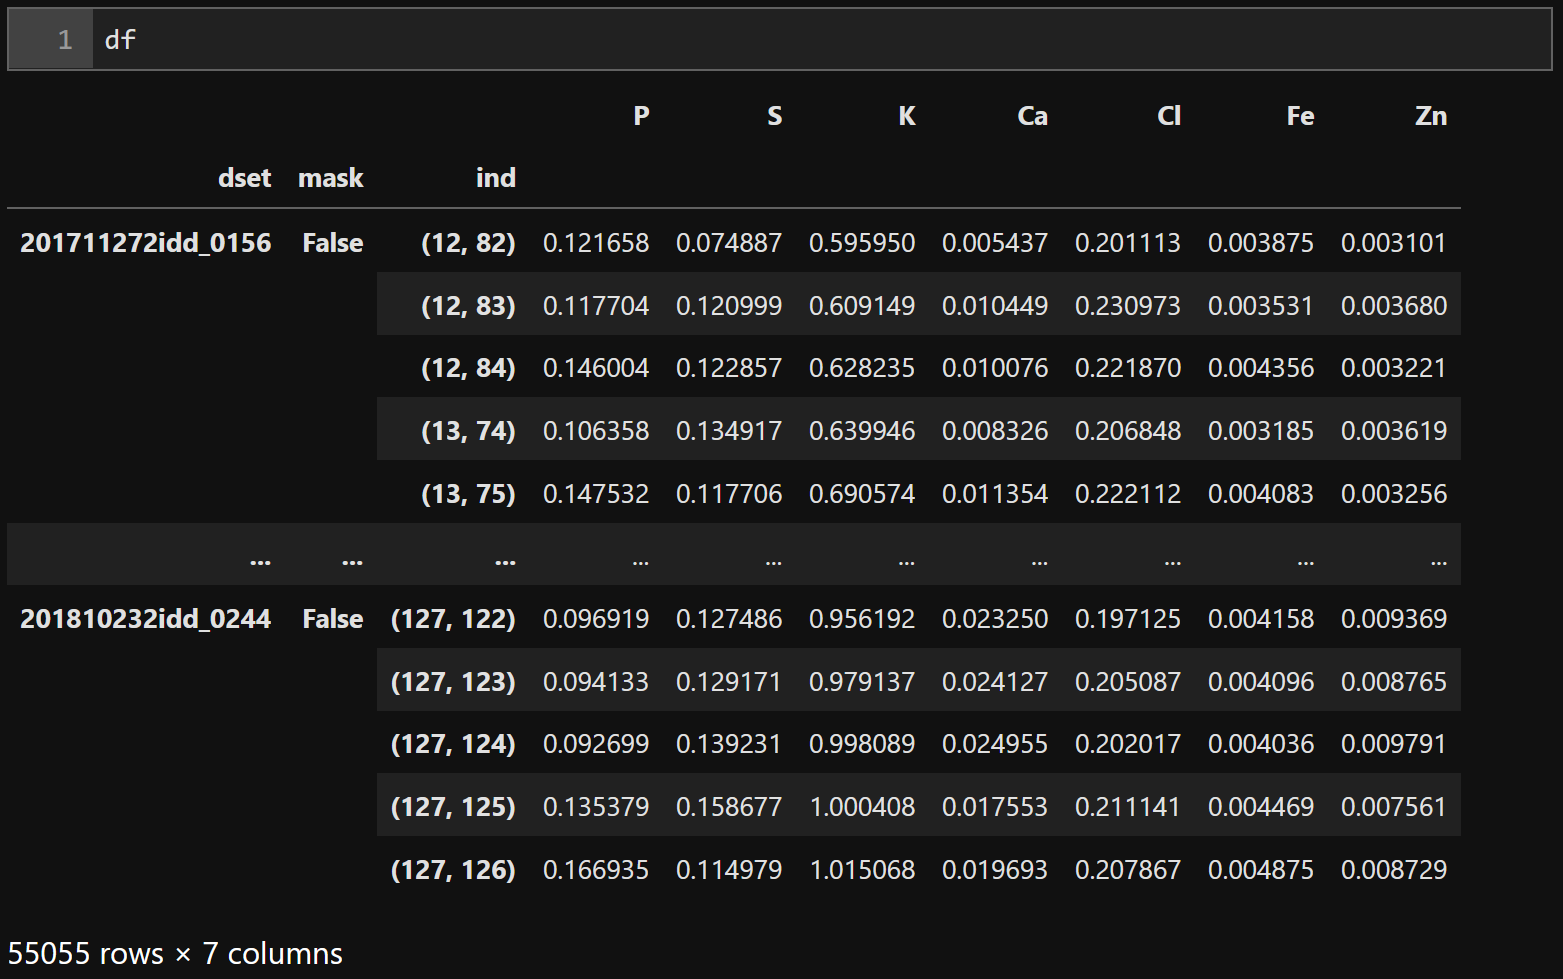
\includegraphics[width=1\textwidth,height=.7\textheight,keepaspectratio]{dataframe.PNG}
    \caption{Multiindex Pandas dataframe for storing data and labels.}
\end{frame}

%page 6
\begin{frame}{3-D projections of 7-D data.}
\begin{figure}[h]
  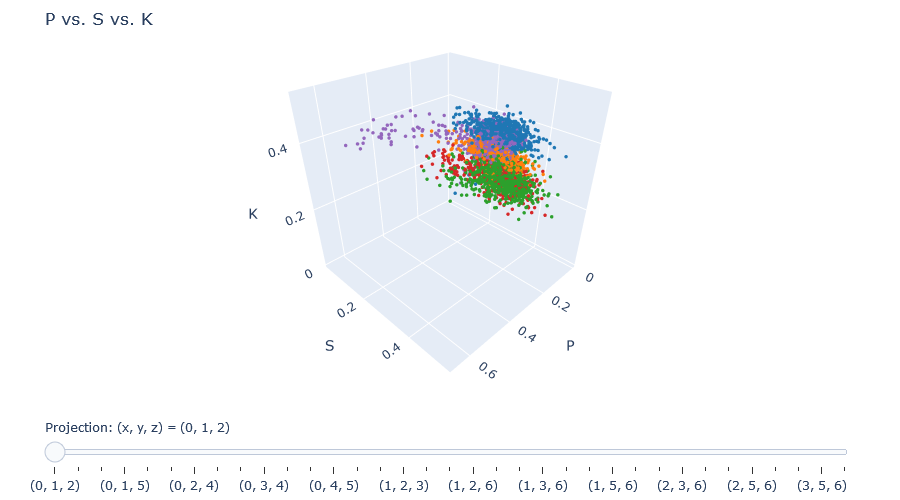
\includegraphics[width=1\textwidth,height=1\textheight,keepaspectratio]{7dto3d.png}
  \caption{XRF images of mouse fibroblasts.}
\end{figure}
\end{frame}

%page 7
\begin{frame}{Results and why to preprocess data.}
\begin{figure}[h]
  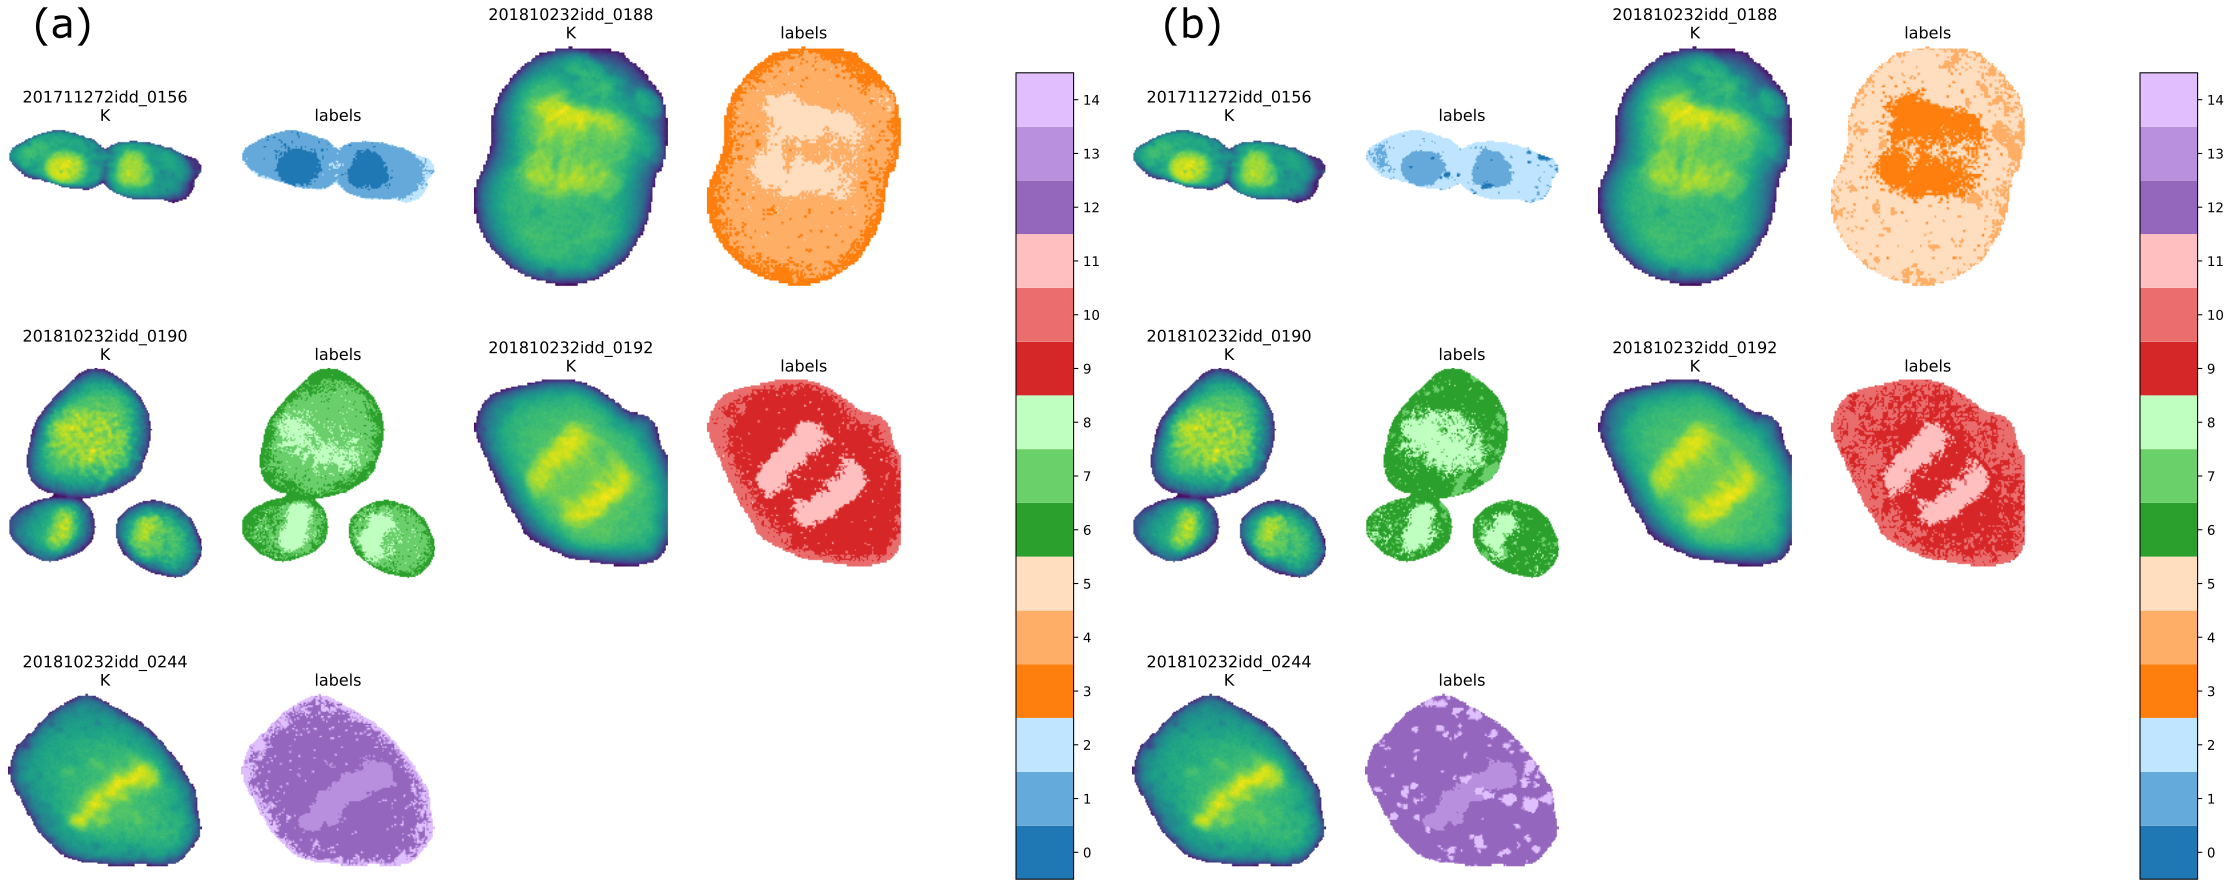
\includegraphics[width=1\textwidth,height=.7\textheight,keepaspectratio]{labels_compare_preprocessing.png}
  \caption{Side by side of potassium channel and labeled regions for two different preprocessing methods. Left: No preprocessing applied, right: robust scaler preprocessing rescales element values to the interquartile range.}
\end{figure}
\end{frame}

\begin{frame}{Pandas results.}
    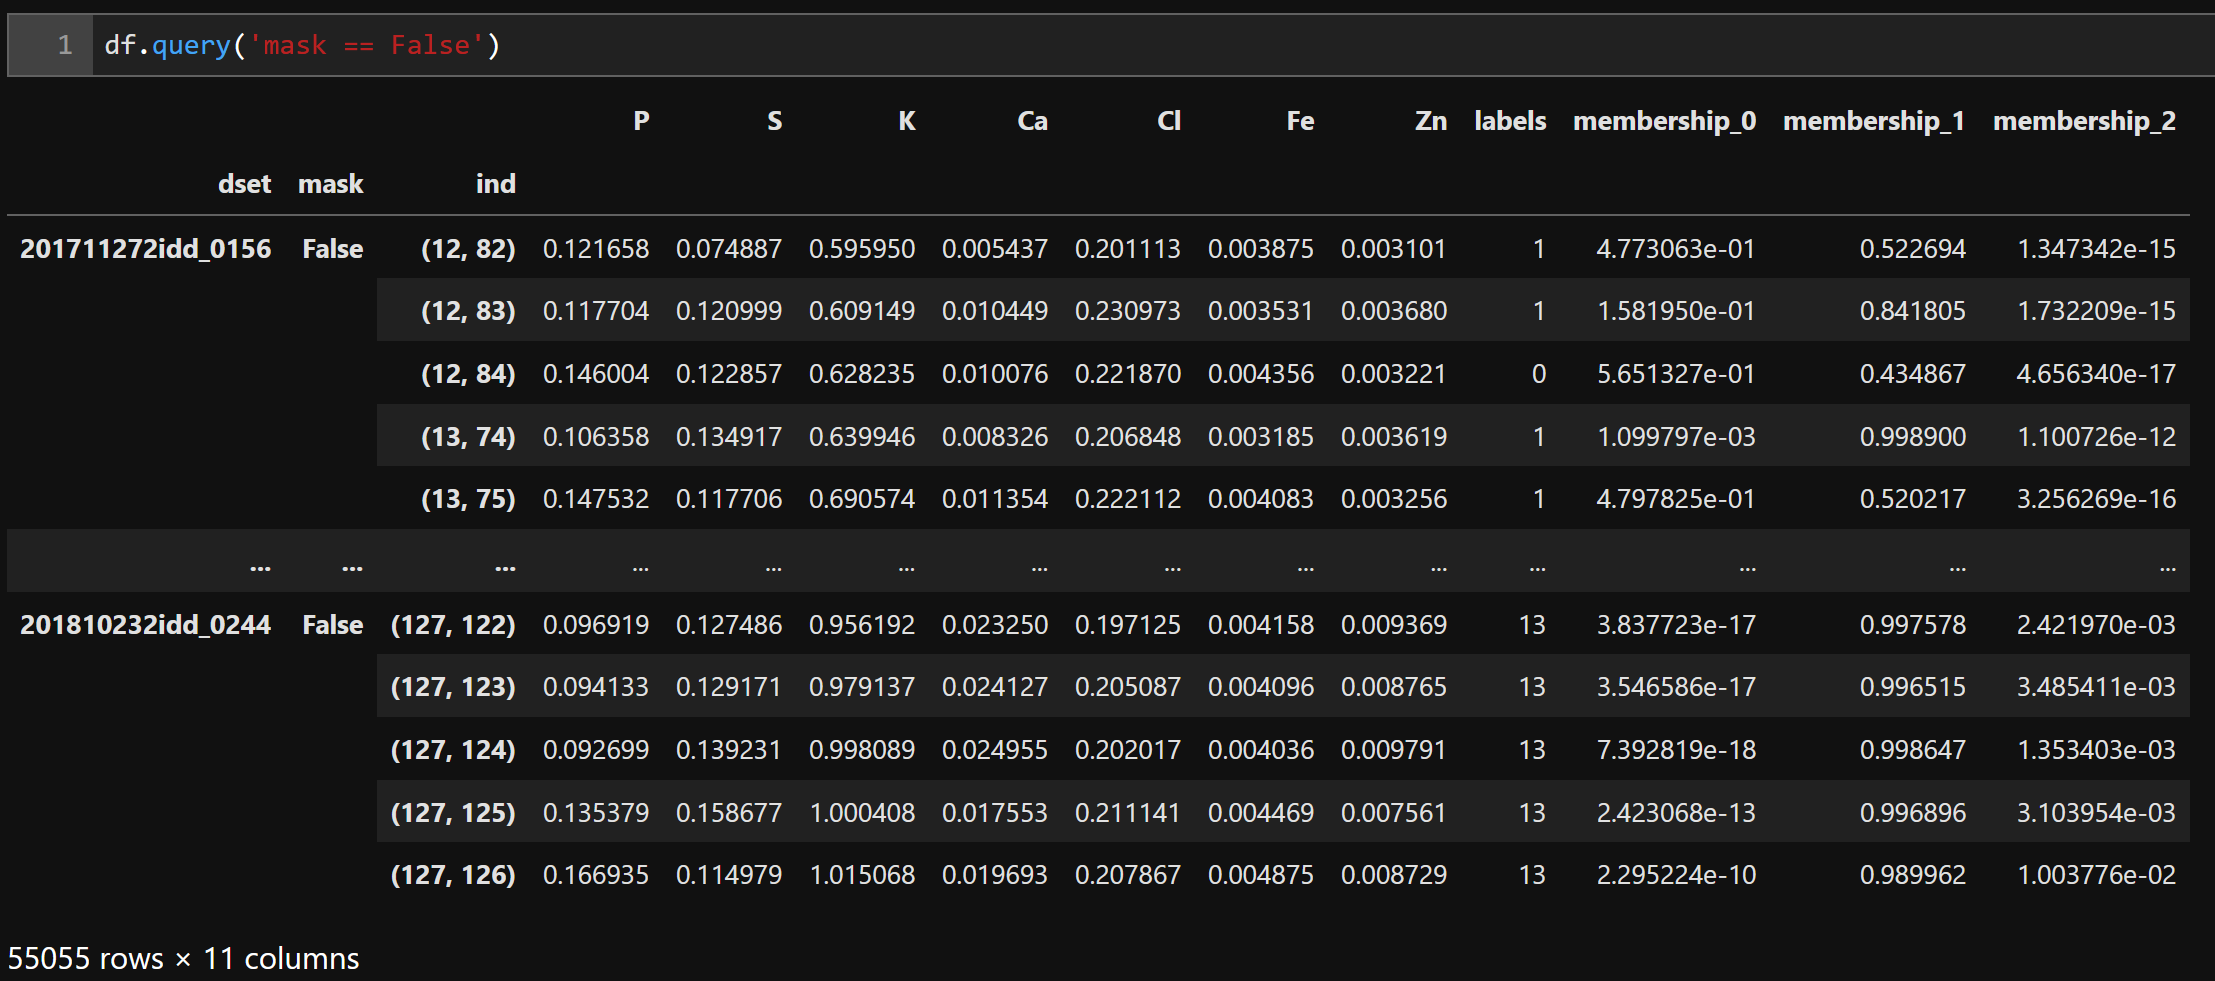
\includegraphics[width=1\textwidth,height=.7\textheight,keepaspectratio]{dataframe_labeled.PNG}
    \caption{Dataframe with labels and membership.}
\end{frame}

%page 9
\begin{frame}{Cluster statistics: Median.}
\begin{figure}[h]
  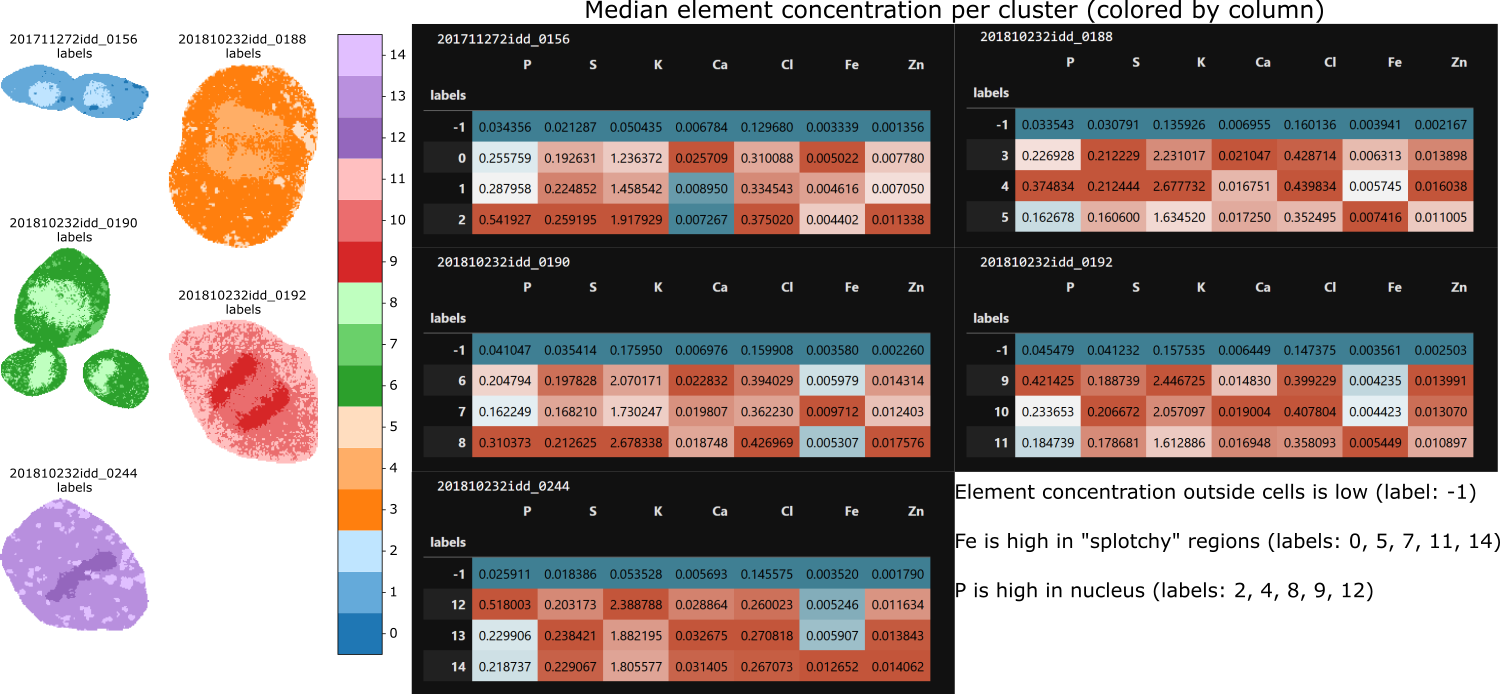
\includegraphics[width=1\textwidth,height=.5\textheight,keepaspectratio]{Cluster_median.png}
  \caption{Median element concentration per cluster.}
\end{figure}
\begin{itemize}
\item Mean, median, standard deviation, correlation coefficient, intraclass correlation, etc... (looking for suggestions)
\item Weighted statistics:
\begin{itemize}
	\item Cluster membership from vMF clustering.
    \item TFY as weight.
\end{itemize}
\end{itemize}
\end{frame}

\begin{frame}{Cluster statistics: Correlation.}
\begin{figure}
    \centering
    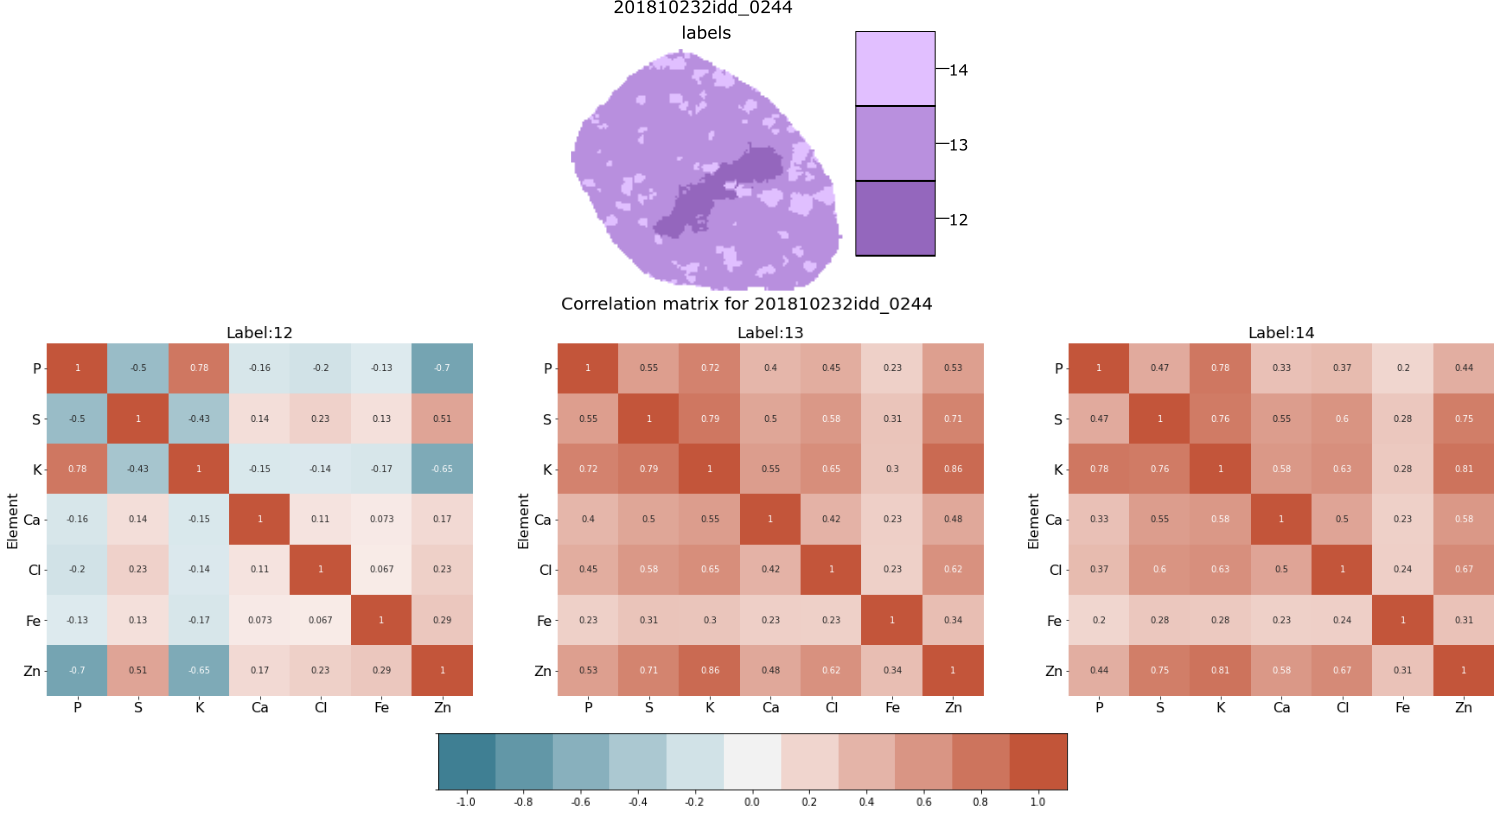
\includegraphics[width=1\textwidth,height=1\textheight,keepaspectratio]{Cluster_corr.png}
    \caption{Cluster correlations for cell \_244.}
    \label{fig:my_label}
\end{figure}
\end{frame}

\begin{frame}{Warning: construction ahead.}
    Everything beyond this point is a work in progress.
\end{frame}

%page 10
\begin{frame}{Extension to 3 spatial dimensions.}
From the perspective of vMF clustering the extension from 2D to 3D is trivial. Each pixel is represented as a vector independent of its location in the dataset. Therefore the clustering algorithm does not care how many spatial dimensions exist. Some clustering algorithms (SLIC) include proximity as a constraint and need to be fed pixel/voxel indicies, but this has been done.
\end{frame}

%page 11
\begin{frame}{Other clustering methods to look into.}
\begin{itemize}
    \item Simple Linear Iterative Clustering (SLIC)
    \item Non-parametric methods (Yang et al.)
    \item Self organizing maps
    \begin{itemize}
        \item Neural gas.
    \end{itemize}
    \item Dimensionality reduction (t-SNE and umap)
\end{itemize}
\end{frame}

%page 12
\begin{frame}{Future.}
\begin{itemize}
    \item Clusters to polygons. This would be especially useful for 3d clustering visualization for viewing embedded organelles, or for importing geometries with material properties into CAD software (for mechanical or semiconductor samples).
    \item Pandas to Dask. Dask is a pandas like framework for big data to be used on supercomputing clusters. One short coming of Dask is a lack of multiindexing (used here for labeling data sets, pixel indicies, and masks). This is an active open issue on their github.
    \item Saving to HDF5 files for sharing.
\end{itemize}
\end{frame}


\section{\bibname}
\begin{frame}[t, allowframebreaks]{\bibname}
\printbibliography[heading=none]
\end{frame}

\begin{frame}[plain]
\vfill
\centerline{Thank You for Your Attention!}
\vfill\vfill
\end{frame}

\end{document}